%
%===============>>  ГРУППА 9-3 МОДУЛЬ 9  <<=============
%
\setmodule{9}

%BEGIN_FOLD % ====>>_____ Занятие 1 _____<<====
\begin{class}[number=1]
	\begin{listofex}
		\item Вычислите:
		\begin{tasks}(2)
			\task \( \left( -\dfrac{ 5 }{ 10 } \right)+4 \cdot (-5) \)
			\task \( (-12 \cdot 0,4) \cdot 0,5 - 11 \)
			\task \( (-25 \cdot \dfrac{ 1 }{ 5 } - 30) \cdot \dfrac{ 1 }{ 7 } \)
			\task \( -\mfrac{3}{5}{21}+\mfrac{3}{17}{42}+\left(-\mfrac{18}{45}{66}\right) \)
			\task \( -15,2 + \left(-\mfrac{2}{17}{25}\right) + 12 \)
			\task \( -\mfrac{4}{2}{3} + \left(-\dfrac{22}{24}\right) - (-6) \)
		\end{tasks}
		\item Найдите значение выражений:
		\begin{tasks}(4)
			\task \( \dfrac{3^7}{81} \)
			\task \( \dfrac{27^5}{9^6} \)
			\task \( \dfrac{81^5}{27^6} \)
			\task \( \dfrac{125^6}{25^8} \)
			\task \( \dfrac{10^6}{2^5\cdot5^4} \)
			\task \( \dfrac{24^4}{3^2\cdot8^3} \)
			\task \( \dfrac{(3\cdot10)^8}{3^6\cdot10^7} \)
			\task \( \dfrac{(2\cdot3)^5}{2^4\cdot3^3} \)
		\end{tasks}
		\item Чему равно значение выражений?
		\begin{tasks}(3)
			\task \( (3\sqrt{2})^2 \)
			\task \( (5\sqrt{3})^2 \)
			\task \( (2\sqrt{7})^2 \)
		\end{tasks}
		\item Найдите значение выражения \( \dfrac{a^{23}\cdot(b^5)^4}{(a\cdot b)^{20}} \) при \( a=2 \) и \( b=\sqrt{2} \).
		\item Найдите значение выражения \( \dfrac{a^{17}\cdot(b^5)^3}{(a\cdot b)^{15}} \) при \( a=7 \) и \( b=\sqrt{7} \).
		\item Найдите значение выражений:
		\begin{tasks}(3)
			\task \( 5\sqrt{11}\cdot2\sqrt{2}\cdot\sqrt{22} \)
			\task \( \sqrt{4\cdot12}\cdot\sqrt{21} \)
			\task \( \sqrt{2\cdot45}\cdot\sqrt{10} \)
			\task \( 3\sqrt{19}\cdot4\sqrt{2}\cdot\sqrt{38} \)
			\task \( 3\sqrt{11}\cdot4\sqrt{2}\cdot\sqrt{22} \)
			\task \( \sqrt{45}\cdot\sqrt{605} \)
		\end{tasks}
	\end{listofex}
\end{class}
%END_FOLD

%BEGIN_FOLD % ====>>_____ Занятие 2 _____<<====
\begin{class}[number=2]
	\begin{listofex}
		\item Решите уравнения:
		\begin{tasks}(2)
			\task \( 7+9(4x+5)=-2 \)
			\task \( 9+2(3-4x)=3x-3 \)
			\task \( x+7-\dfrac{x}{3}=3 \)
			\task \( 1+\dfrac{x}{7}=x+7 \)
		\end{tasks}
		\item Найдите значение выражения \( a^{12}\cdot(a^{-4})^4 \) при \( a=-\dfrac{1}{2} \).
		\item Найдите значение выражения:
		\begin{tasks}(4)
			\task \( \dfrac{(2\cdot5)^6}{2^4\cdot5^5} \)
			\task \( \dfrac{(5\cdot7)^6}{5^4\cdot7^6} \)
			\task \( \dfrac{15^8}{3^6\cdot5^7} \)
			\task \( \dfrac{10^6}{2^5\cdot5^4} \)
		\end{tasks}
		\item Длину окружности \( l \) можно вычислить по формуле \( l=2\pi R \), где \( R \) --- радиус окружности (в метрах). Пользуясь этой формулой, найдите радиус окружности, если её длина равна \( 78 \) м. (Считать \( \pi=3 \)).
		\item Площадь ромба \( S \) (в м\( ^2 \))  можно вычислить по формуле \( S=\dfrac{1}{2}d_1d_2 \),  где \( d_1 \), \( d_2 \) --- диагонали ромба (в метрах). Пользуясь этой формулой, найдите диагональ \( d_1 \), если диагональ \( d_2 \) равна \( 30 \) м, а площадь ромба \( 120 \) м\( ^2 \).
		\item Площадь треугольника \( S \) (в м\( ^2 \)) можно вычислить по формуле \( S=\dfrac{1}{2}ah \),  где a\( a \) --- сторона треугольника, \( h \) --- высота, проведенная к этой стороне (в метрах). Пользуясь этой формулой, найдите сторону \( a \), если площадь треугольника равна \( 28 \) м\( ^2 \), а высота \( h \) равна \( 14 \) м.
		\item Площадь трапеции \( S \) (в м\( ^2 \)) можно вычислить по формуле \( S=\dfrac{a+b}{2}\cdot h \),  где \( a \), \( b \) --- основания трапеции, \( h \) --- высота (в метрах). Пользуясь этой формулой, найдите высоту \( h \), если основания трапеции равны \( 5 \) м и \( 7 \) м, а её площадь \( 24 \) м\( ^2 \).
		\item Объём пирамиды вычисляют по формуле \(V=\dfrac{ 1 }{ 3 }Sh\),  где \(S\) --- площадь основания пирамиды, \(h\) --- её высота. Объём пирамиды равен \(40\), площадь основания \(15\). Чему равна высота пирамиды?
		\item Найдите значение выражений:
		\begin{tasks}(3)
			\task \( 5\sqrt{11}\cdot2\sqrt{2}\cdot\sqrt{22} \)
			\task \( \sqrt{4\cdot12}\cdot\sqrt{21} \)
			\task \( \sqrt{2\cdot45}\cdot\sqrt{10} \)
			\task \( 3\sqrt{19}\cdot4\sqrt{2}\cdot\sqrt{38} \)
			\task \( 3\sqrt{11}\cdot4\sqrt{2}\cdot\sqrt{22} \)
			\task \( \sqrt{45}\cdot\sqrt{605} \)
		\end{tasks}
	\end{listofex}
\end{class}
%END_FOLD

%BEGIN_FOLD % ====>>_ Домашняя работа 1 _<<====
\begin{homework}[number=1]	
	\begin{listofex}
		\item Вычислите:
		\begin{tasks}(2)
			\task \( \dfrac{7,2-6,1}{2,2} \)
			\task \( \dfrac{11}{4,4\cdot2,5} \)
			\task \( \left( \dfrac{7}{25}+\dfrac{7}{33} \right):\dfrac{14}{33} \)
			\task \( \left( \dfrac{17}{25}-\dfrac{1}{17} \right)\cdot\dfrac{17}{4} \)
		\end{tasks}
		\item Вычислите:
		\begin{tasks}(4)
			\task \( 3^{-7}\cdot(3^5)^2 \)
			\task \( \dfrac{(2\cdot6)^7}{2^5\cdot6^6} \)
			\task \( \dfrac{32^5}{8^8} \)
			\task \( \dfrac{6^7}{2^6\cdot3^5} \)
		\end{tasks}
		\item Вычислите:
		\begin{tasks}(2)
			\task \( \sqrt{40\cdot60\cdot75} \)
			\task \( 2\sqrt{11}\cdot2\sqrt{3}\cdot\sqrt{33} \)
			\task \( 4\sqrt{30}\cdot2\sqrt{2}\cdot\sqrt{60} \)
			\task \( 4\sqrt{15}\cdot2\sqrt{5}\cdot\sqrt{75} \)
		\end{tasks}
		\item Решите уравнения:
		\begin{tasks}(1)
			\task \( -3x+1-36(x+3)=-2(1-x)+2 \)
			\task \( -5x-2+4(x+1)=4(-3-x)-1 \)
		\end{tasks}
		\item Зная длину своего шага, человек может приближённо подсчитать пройденное им расстояние \( s \) по формуле \( s=nl \), где \( n \) --- число шагов, \( l \) --- длина шага. Какое расстояние прошёл человек, если \( l=80 \) см, \( n=1600 \)? Ответ выразите в километрах.
	\end{listofex}
\end{homework}
%END_FOLD

%BEGIN_FOLD % ====>>_____ Занятие 3 _____<<====
\begin{class}[number=3]
	\begin{listofex}
		\item В фирме «Родник» стоимость (в рублях) колодца из железобетонных колец рассчитывается по формуле \( C=6000+4100\cdot n \), где \( n \) --- число колец, установленных при рытье колодца. Пользуясь этой формулой, рассчитайте стоимость колодца из \( 5 \) колец.
		\item В фирме «Эх, прокачу!» стоимость поездки на такси (в рублях) рассчитывается по формуле \( C=150+11\cdot(t-5) \), где \( t \) --- длительность поездки, выраженная в минутах (\( t>5 \)). Пользуясь этой формулой, рассчитайте стоимость \( 8 \)-минутной поездки.
		\item Радиус вписанной в прямоугольный треугольник окружности можно найти по формуле \( r=\dfrac{a+b-c}{2} \),  где \( a \) и \( b \) --- катеты, а \( c \) --- гипотенуза треугольника. Пользуясь этой формулой, найдите \( b \), если \( r=1,2 \); \( c=6,8 \) и \( a=6 \).
		\item Площадь любого выпуклого четырехугольника можно вычислять по формуле \( S=\dfrac{1}{2}d_1d_2\sin\alpha \),  где \( d_1 \), \( d_2 \) --- длины его диагоналей, а \( \alpha \) угол между ними. Вычислите \( \sin\alpha \), если \( S=21 \), \( d_1=7 \), \( d_2=15 \).
		\item Мощность постоянного тока (в ваттах) вычисляется по формуле \( P=I^2R \), где \( I \) --- сила тока (в амперах), \( R \) --- сопротивление (в омах). Пользуясь этой формулой, найдите сопротивление \( R \) (в омах), если мощность составляет \( 150 \) ватт, а сила тока равна \( 5 \) амперам.
		\item На экзамене \( 25 \) билетов, Сергей не выучил \( 3 \) из них. Найдите вероятность того, что ему попадётся выученный билет.
		\item Телевизор у Маши сломался и показывает только один случайный канал. Маша включает телевизор. В это время по трем каналам из двадцати показывают кинокомедии. Найдите вероятность того, что Маша попадет на канал, где комедия не идет.
		\item На тарелке \( 12 \) пирожков: \( 5 \) с мясом, \( 4 \) с капустой и \( 3 \) с вишней. Наташа наугад выбирает один пирожок. Найдите вероятность того, что он окажется с вишней.
		\item В фирме такси в данный момент свободно \( 20 \) машин: \( 9 \) черных, \( 4 \) желтых и \( 7 \) зеленых. По вызову выехала одна из машин, случайно оказавшаяся ближе всего к заказчику. Найдите вероятность того, что к нему приедет желтое такси.
		\item В каждой десятой банке кофе согласно условиям акции есть приз. Призы распределены по банкам случайно. Варя покупает банку кофе в надежде выиграть приз. Найдите вероятность того, что Варя не найдет приз в своей банке.
		\item Миша с папой решили покататься на колесе обозрения. Всего на колесе двадцать четыре кабинки, из них \( 5 \) --- синие, \( 7 \) --- зеленые, остальные  — красные. Кабинки по очереди подходят к платформе для посадки. Найдите вероятность того, что Миша прокатится в красной кабинке.
		\item У бабушки \( 20 \) чашек: \( 5 \) с красными цветами, остальные с синими. Бабушка наливает чай в случайно выбранную чашку. Найдите вероятность того, что это будет чашка с синими цветами.
		\item Родительский комитет закупил \( 25 \) пазлов для подарков детям на окончание года, из них \( 15 \) с машинами и \( 10 \) с видами городов. Подарки распределяются случайным образом. Найдите вероятность того, что Толе достанется пазл с машиной.
		\item В среднем из каждых \( 80 \) поступивших в продажу аккумуляторов \( 76 \) аккумуляторов заряжены. Найдите вероятность того, что купленный аккумулятор не заряжен.
		\item Для экзамена подготовили билеты с номерами от \( 1 \) до \( 50 \). Какова вероятность того, что наугад взятый учеником билет имеет однозначный номер?
		\item Из \( 900 \) новых флеш-карт в среднем \( 54 \) не пригодны для записи. Какова вероятность того, что случайно выбранная флеш-карта пригодна для записи?
		\item В коробке \( 14 \) пакетиков с чёрным чаем и \( 6 \) пакетиков с зелёным чаем. Павел наугад вынимает один пакетик. Какова вероятность того, что это пакетик с зелёным чаем?
		\item Стас, Денис, Костя, Маша, Дима бросили жребий --- кому начинать игру. Найдите вероятность того, что начинать игру должна будет девочка.
		\item Вычислите:
		\begin{tasks}(2)
			\task \( \sqrt{66\cdot110\cdot15} \)
			\task \( 3\sqrt{19}\cdot3\sqrt{2}\cdot\sqrt{38} \)
			\task \( 2\sqrt{22}\cdot2\sqrt{3}\cdot\sqrt{66} \)
			\task \( 2\sqrt{10}\cdot5\sqrt{6}\cdot\sqrt{60} \)
			\task \( 3\sqrt{13}\cdot3\sqrt{2}\cdot\sqrt{26} \)
			\task \( 2\sqrt{41}\cdot2\sqrt{3}\cdot\sqrt{123} \)
			\task \( 2\sqrt{10}\cdot3\sqrt{3}\cdot\sqrt{30} \)
			\task \( 4\sqrt{11}\cdot4\sqrt{3}\cdot\sqrt{33} \)
			\task \( 2\sqrt{11}\cdot8\sqrt{3}\cdot\sqrt{33} \)
		\end{tasks}
	\end{listofex}
\end{class}
%END_FOLD

%BEGIN_FOLD % ====>>_____ Занятие 4 _____<<====
\begin{class}[number=4]
	\begin{listofex}
		\item Занятие 4
	\end{listofex}
\end{class}
%END_FOLD

%BEGIN_FOLD % ====>>_ Домашняя работа 2 _<<====
\begin{homework}[number=2]
	\begin{listofex}
		\item Вычислите:
		\begin{tasks}(2)
			\task \( \sqrt{66\cdot110\cdot15} \)
			\task \( 3\sqrt{19}\cdot3\sqrt{2}\cdot\sqrt{38} \)
			\task \( 2\sqrt{22}\cdot2\sqrt{3}\cdot\sqrt{66} \)
			\task \( 2\sqrt{10}\cdot5\sqrt{6}\cdot\sqrt{60} \)
			\task \( 3\sqrt{13}\cdot3\sqrt{2}\cdot\sqrt{26} \)
			\task \( 2\sqrt{41}\cdot2\sqrt{3}\cdot\sqrt{123} \)
		\end{tasks}
		\item Решите уравнения:
		\begin{tasks}(2)
			\task \( \dfrac{6x+8}{2}+5=\dfrac{5x}{3} \)
			\task \( 6+\dfrac{x}{2}=\dfrac{x+3}{5} \)
		\end{tasks}
		\item Закон Джоуля-Ленца можно записать в виде \( Q=I^2Rt \), где Q --- количество теплоты (в джоулях), \( I \) --- сила тока (в амперах), \( R \) --- сопротивление цепи (в омах), а \( t \) ---  время (в секундах). Пользуясь этой формулой, найдите время \( t \) (в секундах), если \( Q=1521 \)  Дж, \( I=6,5  \) A, \( R=9 \)  Ом.
		\item Закон Менделеева-Клапейрона можно записать в виде \( PV=vRT \), где \( P \) --- давление (в паскалях), \( V \) --- объём (в м\( ^3 \)), \( v \) --- количество вещества (в молях), \( T \) --- температура (в градусах Кельвина), а \( R \) --- универсальная газовая постоянная, равная \( 8,31 \) Дж/(К\( \cdot \)моль). Пользуясь этой формулой, найдите количество вещества \( v \) (в молях), если \( T=700 \) К, \( P=20 941,2 \) Па, \( V=9,5 \) м\( ^3 \).
		\item На экзамене \( 20 \) билетов, Сергей не выучил \( 3 \) из них. Найдите вероятность того, что ему попадётся выученный билет.
		\item Максим с папой решили покататься на колесе обозрения. Всего на колесе двадцать кабинок, из них \( 4 \) --- синие, \( 10 \) --- зеленые, остальные --- красные. Кабинки по очереди подходят к платформе для посадки. Найдите вероятность того, что Максим прокатится в красной кабинке.
		\item Из \( 900 \) новых флеш-карт в среднем \( 54 \) не пригодны для записи. Какова вероятность того, что случайно выбранная флеш-карта пригодна для записи?
		\item В лыжных гонках участвуют \( 13 \) спортсменов из России, \( 2 \) спортсмена из Норвегии и \( 5 \) спортсменов из Швеции. Порядок, в котором спортсмены стартуют, определяется жребием. Найдите вероятность того, что первым будет стартовать спортсмен не из России.
	\end{listofex}
\end{homework}
%END_FOLD

%BEGIN_FOLD % ====>>_____ Занятие 5 _____<<====
\begin{class}[number=5]
	\begin{listofex}
		\item .
	\end{listofex}
\end{class}
%END_FOLD

%BEGIN_FOLD % ====>>_____ Занятие 6 _____<<====
\begin{class}[number=6]
	\begin{listofex}
		\item .
	\end{listofex}
\end{class}
%END_FOLD

%BEGIN_FOLD % ====>>_ Домашняя работа 3 _<<====
\begin{homework}[number=3]
	\begin{listofex}
		\item Вычислите:
		\begin{tasks}(2)
			\task \( \dfrac{6,9-1,5}{2,4} \)
			\task \( \dfrac{2,4}{2,9-1,4} \)
			\task \( \dfrac{9,4}{4,1+5,3} \)
			\task \( \dfrac{6,9+4,1}{0,2} \)
		\end{tasks}
		\item Решите уравнение: \( \dfrac{5x}{9}=\dfrac{1}{8}:\mfrac{3}{3}{4} \)
		\item На экзамене \( 25 \) билетов, Сергей не выучил \( 3 \) из них. Найдите вероятность того, что ему попадётся выученный билет.
		\item Коля выбирает трехзначное число. Найдите вероятность того, что оно делится на \( 5 \).
		\item Телевизор у Маши сломался и показывает только один случайный канал. Маша включает телевизор. В это время по трем каналам из двадцати показывают кинокомедии. Найдите вероятность того, что Маша попадет на канал, где комедия не идет.
		\item На тарелке \( 12 \) пирожков: \( 5 \) с мясом, \( 4 \) с капустой и \( 3 \) с вишней. Наташа наугад выбирает один пирожок. Найдите вероятность того, что он окажется с вишней.
		\item В каждой десятой банке кофе согласно условиям акции есть приз. Призы распределены по банкам случайно. Варя покупает банку кофе в надежде выиграть приз. Найдите вероятность того, что Варя не найдет приз в своей банке.
		\item Найдите значение выражений:
		\begin{tasks}(2)
			\task \( \sqrt{2^2\cdot5^4\cdot49^2} \)
			\task \( 3\sqrt{19}\cdot3\sqrt{2}\cdot\sqrt{38} \)
			\task \( \sqrt{13\cdot18}\cdot\sqrt{26} \)
			\task \( (\sqrt{37}-5)(\sqrt{37}+5) \)
			\task \( (\sqrt{27}+\sqrt{3})\cdot\sqrt{3} \)
			\task \( (5+\sqrt{2})^2+(5-\sqrt{2})^2 \)
		\end{tasks}
	\end{listofex}
\end{homework}
%END_FOLD

%BEGIN_FOLD % ====>>_____ Занятие 7 _____<<====
\begin{class}[number=7]
	\begin{listofex}
		\item Найдите значение выражения: \((4,9\cdot10^{-3})(4\cdot10^{-2})\).
		\item На координатной прямой отмечены числа \( a \) и \( b \). Какое из следующих утверждений неверно?
		\begin{center}
			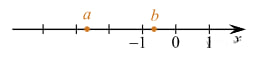
\includegraphics[align=t, width=0.5\linewidth]{\picpath/G93M8L6-6}
		\end{center}
		\begin{tasks}(2)
			\task \( a+b<0 \)
			\task \( -2<b-1<-1 \)
			\task \( a^2b<0 \)
			\task \( -a<0 \)
		\end{tasks}
		\item Найдите значение выражения \( \dfrac{a^2-25b^2}{5ab}:\left( \dfrac{1}{5b}-\dfrac{1}{a} \right) \) при \( a=\mfrac{8}{1}{16} \), \( b=\mfrac{6}{3}{16} \).
		\item Решите уравнениe: \((x-11)(-x+9)=0\).
		\item Определите вероятность того, что при бросании игрального кубика (правильной кости) выпадет более \( 3 \) очков.
		\item Установите соответствие между графиками функций и формулами, которые их задают.
		\begin{center}
			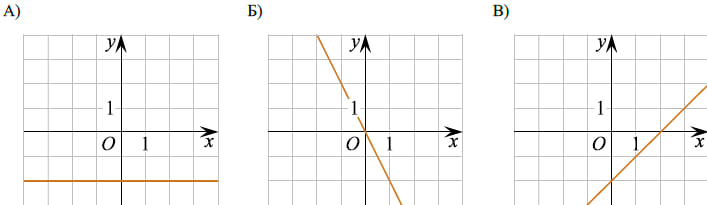
\includegraphics[align=t, width=0.7\linewidth]{\picpath/G91M9L5}
		\end{center}
		\begin{tasks}(3)
			\task \( y=-2 \)
			\task \( y=x-2 \)
			\task \( y=-2x \)
		\end{tasks}
		\item Закон всемирного тяготения можно записать в виде \( F=y\dfrac{m_1m_2}{r^2} \) где \( F \) --- сила притяжения между телами (в ньютонах), \( m_1 \) и \( m_2 \) --- массы тел (в килограммах), \( r \) --- расстояние между центрами масс (в метрах), а \( y \) --- гравитационная постоянная, равная \( 6,67\cdot10^{-11} \) H\( \cdot \)м\( ^2 \)/кг\( ^2 \). Пользуясь формулой, найдите массу тела (в килограммах), если \( F=1000,5 \) Н, \( m_2=6\cdot10^9 \) кг, а \( r=4 \) м.
		\item Решение какого из данных неравенств изображено на рисунке?
		\begin{center}
			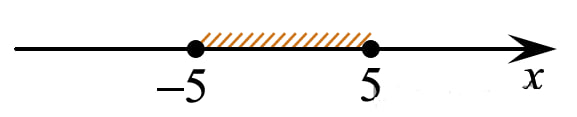
\includegraphics[align=t, width=0.5\linewidth]{\picpath/G91M9L5-1}
		\end{center}
		\begin{tasks}(4)
			\task \( x^2-25\le0 \)
			\task \( x^2+25\le0 \)
			\task\( x^2-25\ge0 \)
			\task \( x^2+25\ge0 \)
		\end{tasks}
		\item В амфитеатре \( 23 \) ряда, причём в каждом следующем ряду на одно и то же число мест больше, чем в предыдущем. В седьмом ряду \( 26 \) мест,	а в одиннадцатом ряду \( 34 \) места. Сколько мест в последнем ряду амфитеатра?
		\item В треугольнике \( ABC \) проведена биссектриса \( AL \), угол \( ALC \) равен \( 112\degree \), угол \( ABC \) равен \( 106\degree \). Найдите угол \( ACB \). Ответ дайте в градусах.
		\item Окружность с центром в точке \( O \) описана около равнобедренного треугольника \( ABC \), в котором \( AB=BC \) и \( \angle ABC=79\degree \). Найдите величину угла \( BOC	 \). Ответ дайте в градусах.
		\item Сторона треугольника равна \( 14 \), а высота, проведённая к этой стороне, равна \( 31 \). Найдите площадь этого треугольника.
		\item
		\begin{minipage}[t]{\bodywidth}
			На клетчатой бумаге с размером клетки \( 1X1 \) изображён параллелограмм. Найдите его площадь.
		\end{minipage}
		\gapwidth
		\begin{minipage}[t]{\picwidth}
			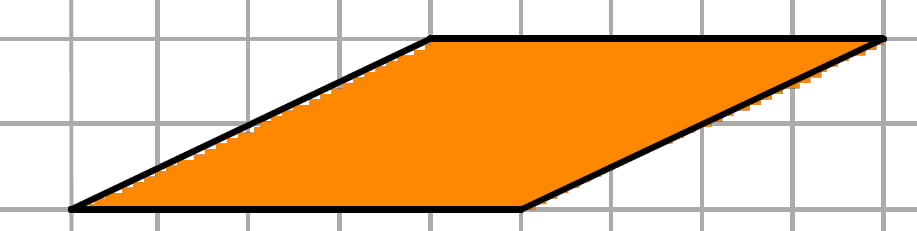
\includegraphics[align=t, width=\linewidth]{\picpath/G91M9L5-3}
		\end{minipage}
		\item Укажите номера верных утверждений.
		\begin{tasks}
			\task Если два угла одного треугольника равны двум углам другого треугольника, то такие треугольники подобны.
			\task Вертикальные углы равны.
			\task Любая биссектриса равнобедренного треугольника является его медианой.
		\end{tasks}
		\item Найдите значение выражения: \(\left( \dfrac{ 17 }{ 15 }-\dfrac{ 1 }{ 12 }\right)\cdot5 \).
		\item Какому промежутку принадлежит число \(\sqrt{66}\)?
		\begin{tasks}(4)
			\task \( [7;\,8] \)
			\task \( [8;\,9] \)
			\task \( [9;\,10] \)
			\task \( [10;\,11] \)
		\end{tasks}
		\item Найдите значение выражения \( \dfrac{(a^7)^3}{a^{18}} \) при \( a=2 \).
		\item Решите уравнение: \( x^2=2x+8 \)
		\item В среднем из каждых \(200\) поступивших в продажу аккумуляторов \(196\) аккумуляторов заряжены. Найдите вероятность того, что купленный аккумулятор не заряжен.
		\item На рисунке изображены графики функций вида \(ax^2+bx+c\). Установите соответствие между графиками функций и знаками коэффициентов \(a\) и \(c\).
		\begin{center}
			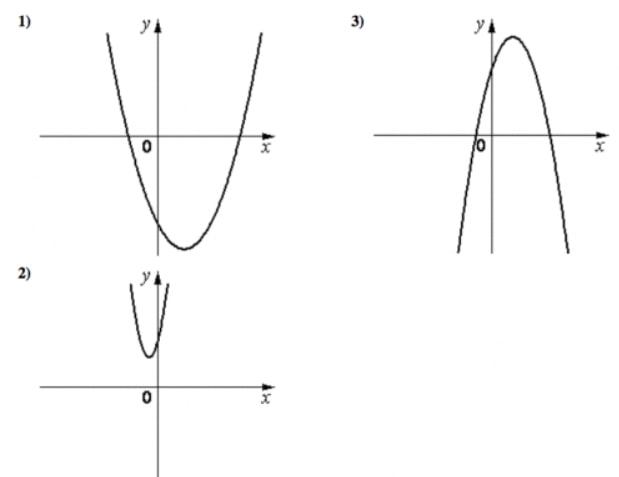
\includegraphics[align=t, width=0.7\linewidth]{\picpath/G91M9L4}
		\end{center}
		\begin{tasks}
			\task \( a>0, c>0 \)
			\task \( a<0, c>0 \)
			\task \( a>, c<0 \)
		\end{tasks}
		\item Закон Менделеева-Клапейрона можно записать в виде \(PV=vRT\), где \(P\) --- давление (в паскалях), \(V\) --- объём (в м\(^3\)), \(v\)  --- количество вещества (в молях), \(T\) --- температура (в градусах Кельвина), а \(R\) --- универсальная газовая постоянная, равная \(8,31\) Дж/(К\(\cdot\) моль). Пользуясь этой формулой, найдите температуру \(T\) (в градусах Кельвина), если \(v=68,2\) моль, \(P=37 782,8\) Па, \(V=6\) м\(^3\).
		\item Решите неравенство: \(x^2+x\le0\).
		\item Васе надо решить \(434\) задачи. Ежедневно он решает на одно и то же количество задач больше по сравнению с предыдущим днем. Известно, что за первый день Вася решил \(5\) задач. Определите, сколько задач решил Вася в последний день, если со всеми задачами он справился за \(14\) дней.
		\item Площадь ромба равна \( 54 \), а периметр равен \( 36 \). Найдите высоту ромба.
		\item Точки \(A\) и \(B\) делят окружность на две дуги, длины которых относятся как \(9:11\). Найдите величину центрального угла, опирающегося на меньшую из дуг. Ответ дайте в градусах.
		\item Найдите площадь прямоугольника, если его периметр равен \(44\) и одна сторона на \(2\) больше другой.
		\item На клетчатой бумаге с размером клетки \( 1 \) см \( X \) \( 1 \) см изображена трапеция. Найдите её площадь. Ответ дайте в квадратных сантиметрах.
		\begin{center}
			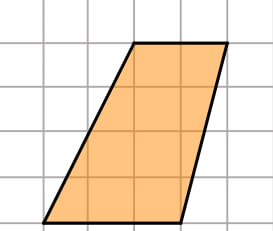
\includegraphics[align=t, width=0.5\linewidth]{\picpath/G93M9L7}
		\end{center}
		\item Укажите номера верных утверждений.
		\begin{tasks}
			\task  Биссектриса равнобедренного треугольника, проведённая из вершины, противолежащей основанию, делит основание на две равные части.
			\task В любом прямоугольнике диагонали взаимно перпендикулярны.
			\task Для точки, лежащей на окружности, расстояние до центра окружности равно радиусу.
		\end{tasks}
	\end{listofex}
\end{class}
%END_FOLD

%BEGIN_FOLD % ====>>_ Проверочная работа _<<====
\begin{class}[number=8]
	\begin{listofex}
		\item Найдите значение выражения: \(\left( \dfrac{ 17 }{ 15 }-\dfrac{ 1 }{ 12 }\right)\cdot5 \).
		\item Какому промежутку принадлежит число \(\sqrt{66}\)?
		\begin{tasks}(4)
			\task \( [7;\,8] \)
			\task \( [8;\,9] \)
			\task \( [9;\,10] \)
			\task \( [10;\,11] \)
		\end{tasks}
		\item Найдите значение выражения \( \dfrac{(a^7)^3}{a^{18}} \) при \( a=2 \).
		\item Решите уравнение: \( x^2=2x+8 \)
		\item В среднем из каждых \(200\) поступивших в продажу аккумуляторов \(196\) аккумуляторов заряжены. Найдите вероятность того, что купленный аккумулятор не заряжен.
		\item На рисунке изображены графики функций вида \(ax^2+bx+c\). Установите соответствие между графиками функций и знаками коэффициентов \(a\) и \(c\).
		\begin{center}
			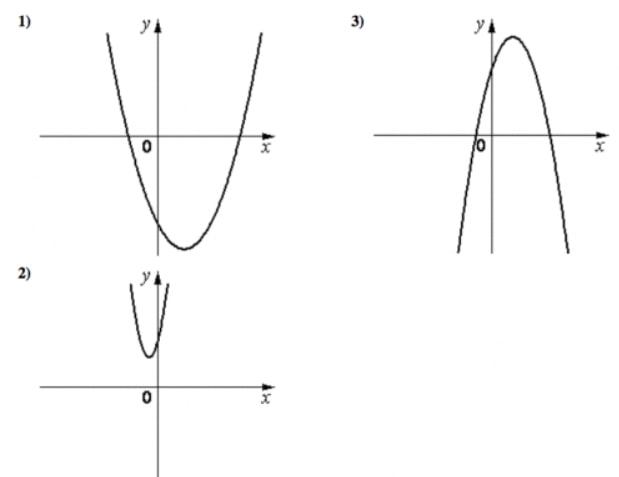
\includegraphics[align=t, width=0.7\linewidth]{\picpath/G91M9L4}
		\end{center}
		\begin{tasks}
			\task \( a>0, c>0 \)
			\task \( a<0, c>0 \)
			\task \( a>, c<0 \)
		\end{tasks}
		\item Закон Менделеева-Клапейрона можно записать в виде \(PV=vRT\), где \(P\) --- давление (в паскалях), \(V\) --- объём (в м\(^3\)), \(v\)  --- количество вещества (в молях), \(T\) --- температура (в градусах Кельвина), а \(R\) --- универсальная газовая постоянная, равная \(8,31\) Дж/(К\(\cdot\) моль). Пользуясь этой формулой, найдите температуру \(T\) (в градусах Кельвина), если \(v=68,2\) моль, \(P=37 782,8\) Па, \(V=6\) м\(^3\).
		\item Решите неравенство: \(x^2+x\le0\).
		\item Васе надо решить \(434\) задачи. Ежедневно он решает на одно и то же количество задач больше по сравнению с предыдущим днем. Известно, что за первый день Вася решил \(5\) задач. Определите, сколько задач решил Вася в последний день, если со всеми задачами он справился за \(14\) дней.
		\item Площадь ромба равна \( 54 \), а периметр равен \( 36 \). Найдите высоту ромба.
		\item Точки \(A\) и \(B\) делят окружность на две дуги, длины которых относятся как \(9:11\). Найдите величину центрального угла, опирающегося на меньшую из дуг. Ответ дайте в градусах.
		\item Найдите площадь прямоугольника, если его периметр равен \(44\) и одна сторона на \(2\) больше другой.
		\item На клетчатой бумаге с размером клетки \( 1 \) см \( X \) \( 1 \) см изображена трапеция. Найдите её площадь. Ответ дайте в квадратных сантиметрах.
		\begin{center}
			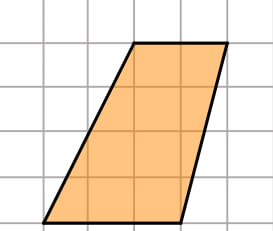
\includegraphics[align=t, width=0.5\linewidth]{\picpath/G93M9L7}
		\end{center}
		\item Укажите номера верных утверждений.
		\begin{tasks}
			\task  Биссектриса равнобедренного треугольника, проведённая из вершины, противолежащей основанию, делит основание на две равные части.
			\task В любом прямоугольнике диагонали взаимно перпендикулярны.
			\task Для точки, лежащей на окружности, расстояние до центра окружности равно радиусу.
		\end{tasks}
	\end{listofex}
\end{class}
%END_FOLD

%BEGIN_FOLD % ====>>_ Проверочная работа _<<====
\begin{class}[number=9]
	\begin{listofex}
\item Найдите значение выражения \( 7,8 + 8,9 \).
\item На координатной прямой отмечено число \( a \). Какое из утверждений для этого числа
является верным?
\begin{figure}[h]
	\center{
		% TODO: \usepackage{graphicx} required
		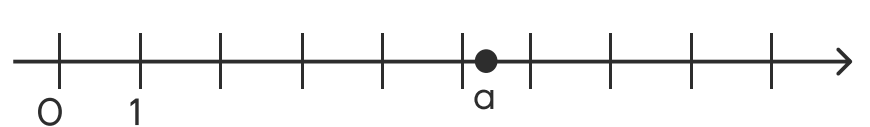
\includegraphics[align=t, width=0.3\linewidth]{../../../../../exercises/lists/pics/leontevaM9H2-7}
	}
\end{figure}
\begin{tasks}(4)
	\task \( 4 - a > 0 \)
	\task \( a-7 < 0 \)
	\task \( a-8 > 0 \)
	\task \( 8 - a > 0 \)
\end{tasks}
\item Найдите значение выражения \( \dfrac{a^{5}\cdot a^{17}}{a^{19}} \) при \( a=2 \).
\item Решите уравнение \( \dfrac{x+3}{x+4}=3 \)
\item В среднем из \( 100 \) карманных фонариков, поступивших в продажу, четыре
неисправных. Найдите вероятность того, что выбранный наудачу в магазине
фонарик окажется исправен.
\item Изображены графики функций \( y = ax^{2} + bx + c \). Сопоставьте графики со знаками
коэффициентов \( a \) и \( c \).
\begin{figure}[h]
	\center{
		% TODO: \usepackage{graphicx} required
		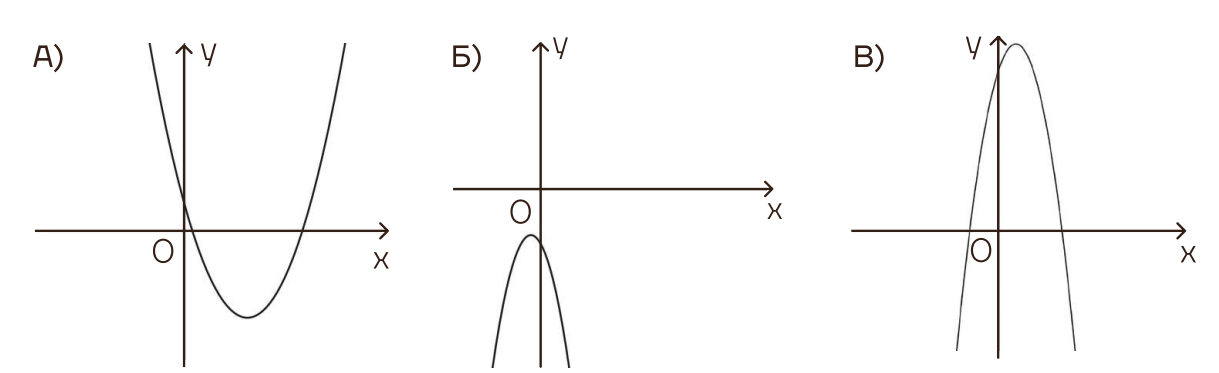
\includegraphics[align=t, width=\linewidth]{../../../../../exercises/lists/pics/leontevaM9H2-8}
	}
\end{figure}
\begin{tasks}(3)
	\task \( a<0 \), \( c>0 \)
	\task \( a>0 \), \( c>0 \)
	\task \( a<0 \), \( c<0 \)
\end{tasks}
\item Мощность постоянного тока (в ваттах) вычисляется по формуле \( P = I^{2}R \) , где \( I \) – сила тока (в амперах), \( R \) – сопротивление (в омах). Пользуясь этой формулой, найдите сопротивление \( R \), если мощность составляет \( 15,75 \) Вт, а сила тока равна \( 1,5 \) \( A \). Ответ дайте в омах.
\item Укажите решение неравенства \( (x-5)(x+3)\leq0 \).
\begin{tasks}(2)
	\task \( [-3;+\infty) \)
	\task \( [-3;5] \)
	\task \( (-\infty;-5] \) \( \bigcup \) \( [5;+\infty) \)
	\task \( [5;+\infty) \)
\end{tasks}
\item В амфитеатре \( 14 \) рядов. В первом ряду \( 16 \) мест, а в каждом следующем на \( 2  \) места
больше, чем в предыдущем. Сколько всего мест в амфитеатре?
\item Сторона треугольника равна \( 16 \), а высота, проведённая к этой стороне, равна \( 15 \).
Найдите площадь этого треугольника.
\item 
\begin{minipage}[t]{\bodywidth}
	Центр окружности, описанной около треугольника \( ABC \), лежит на стороне \( AB \). Радиус окружности равен \( 14,5 \). Найдите \( AC \), если \( BC = 21 \).
\end{minipage}
\hspace{0.02\linewidth}
\begin{minipage}[t]{\picwidth}
	% TODO: \usepackage{graphicx} required
	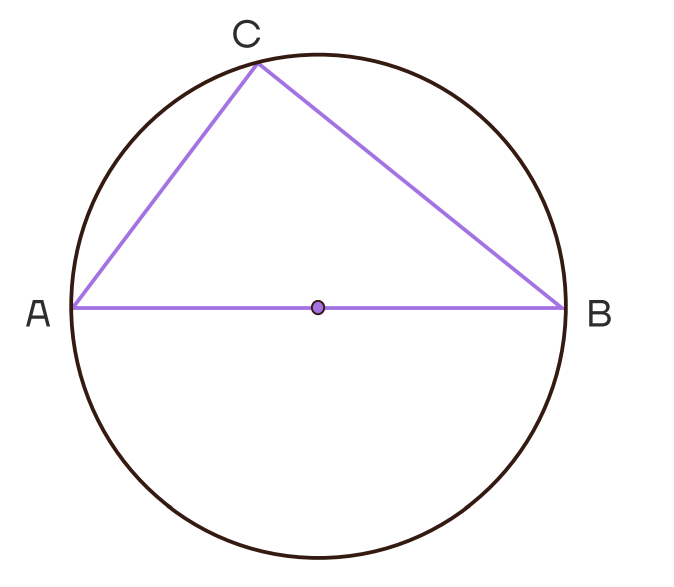
\includegraphics[align=t, width=\linewidth]{../../../../../exercises/lists/pics/leontevaM9H2-10}
\end{minipage}
\item 
\begin{minipage}[t]{\bodywidth}
	В равнобедренной трапеции известна высота, меньшее основание и угол при
	основании (см. рисунок). Найдите большее основание.
\end{minipage}
\hspace{0.02\linewidth}
\begin{minipage}[t]{\picwidth}
	% TODO: \usepackage{graphicx} required
	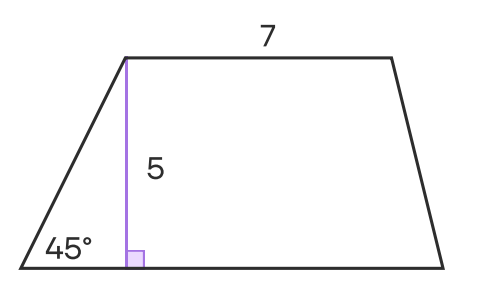
\includegraphics[align=t, width=\linewidth]{../../../../../exercises/lists/pics/leontevaM9H2-9}
\end{minipage}
\item 
\begin{minipage}[t]{\bodywidth}
	На клетчатой бумаге с размером клетки \(  1\times 1 \) изображена трапеция. Найдите
	длину её средней линии.
\end{minipage}
\hspace{0.02\linewidth}
\begin{minipage}[t]{\picwidth}
	% TODO: \usepackage{graphicx} required
	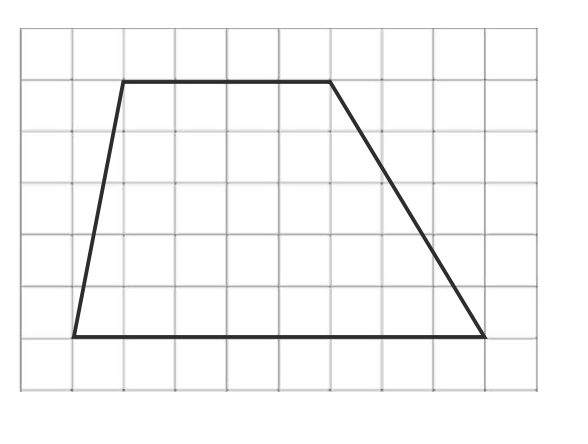
\includegraphics[align=t, width=\linewidth]{../../../../../exercises/lists/pics/leontevaM9H2-11}
\end{minipage}
\item Какие из следующих утверждений верны? \begin{tasks}(1)
	\task В треугольнике против меньшего угла лежит большая сторона.
	
	\task Если один угол треугольника больше \( 120\degree \), то два других его угла меньше \( 30\degree \).
	
	\task Если все стороны треугольника меньше \( 1 \), то и все его высоты меньше \(  1 \).
	
	\task Сумма острых углов прямоугольного треугольника не превосходит \( 90\degree \).
\end{tasks}
	\end{listofex}
\end{class}
%END_FOLD